Este capítulo apresenta como a plataforma foi testada. A Seção~\ref{sec:planejamento-testes} descreve o planejamento: o que se decidiu testar, em quais níveis e com quais ferramentas. As seções seguintes relatam a realização dos testes. A Seção~\ref{sec:testes-unitarios} trata dos testes unitários e de integração da IDE, a Seção~\ref{subsec:e2e-plataforma} dos testes de ponta a ponta, a Seção~\ref{subsec:ci-plataforma} da integração contínua e a Seção~\ref{subsec:resultado-e2e} do resultado da execução local desses testes. A Seção~\ref{subsec:verificacao-interface} descreve a verificação técnica de acessibilidade e responsividade do assistente de personalização. A avaliação da plataforma pelo painel de especialistas não faz parte deste capítulo: seu protocolo está na Seção~\ref{sec:protocolo-avaliacao} e seus resultados, no Capítulo~\ref{cap:resultados}.

As descrições de código deste capítulo referem-se ao repositório do projeto, apresentado no Apêndice~\ref{ap:repositorio}. As contagens de testes aprovados vêm dos registros de execução reunidos no Apêndice~\ref{ap:verificacao}.

\section{Planejamento dos testes}
\label{sec:planejamento-testes}

O planejamento seguiu a pirâmide de testes apresentada na Subseção~\ref{subsec:testes-tdd}: muitos testes pequenos e rápidos na base, que verificam módulos isolados, e menos testes nos níveis superiores, que exercitam a aplicação inteira e são mais lentos e mais caros de manter \cite{vocke2018pyramid}. Cada nível ficou com um objeto, uma ferramenta e uma forma de execução:

\begin{itemize}
    \item Testes unitários: verificam funções e módulos da IDE e do compilador sem interface, como a configuração da linguagem, a validação das personalizações e a persistência no armazenamento local. Usam o \textit{framework} Vitest e ficam, em geral, em arquivos com sufixo \texttt{.spec.ts} ao lado dos módulos que verificam; alguns ficam em diretórios \texttt{\_\_tests\_\_}.
    \item Testes de integração de componentes: verificam componentes React da IDE em conjunto com seus \textit{contexts} e \textit{hooks}, como os componentes do assistente, a depuração e as submissões. Também usam Vitest, com o \textit{jsdom} simulando o ambiente do navegador, e ficam em arquivos com sufixo \texttt{.spec.tsx} próximos aos componentes.
    \item Testes de ponta a ponta (E2E, do inglês \textit{end-to-end}): verificam fluxos completos no navegador, com o front-end, o serviço FastAPI e o banco PostgreSQL em execução. Usam o Playwright Test com o Chromium e ficam no pacote \texttt{packages/e2e}.
    \item Verificação técnica da interface: verifica, na primeira etapa do assistente de personalização, a navegação por teclado, a adaptação a larguras de computador e de celular e as regras de acessibilidade que uma ferramenta automática consegue avaliar. Usa o Playwright para conduzir o navegador e o axe-core para a análise.
\end{itemize}

Os testes unitários, de integração e E2E também foram planejados para rodar na integração contínua do GitHub Actions, que executa ainda os testes do back-end com pytest. A implantação automatizada só ocorre se esses testes forem aprovados. O critério de aprovação, em todos os níveis, é o resultado das asserções de cada caso; na integração contínua, um caso E2E que só passa depois de repetido também reprova a execução, como detalha a Seção~\ref{subsec:ci-plataforma}.

O planejamento não incluiu uma meta de cobertura de código, e nenhum dos níveis mede essa cobertura. Os testes oferecem evidência do comportamento que cobrem e apoio à detecção de regressões. A presença de uma suíte, por si só, não comprova que o ciclo de escrever o teste antes da implementação tenha sido seguido em todos os incrementos.

\section{Testes unitários e de integração}
\label{sec:testes-unitarios}

A revisão de 16 de setembro de 2026 registrou 139 aprovações em 28 arquivos selecionados pelo comando de testes da IDE, além de seis verificações executadas separadamente. Após os merges, a configuração passou a descobrir arquivos \texttt{.spec.ts} e \texttt{.spec.tsx} em toda a árvore de fontes, mantendo oito exclusões explícitas de testes do assistente ainda pendentes de atualização. Em 19 de setembro de 2026, a execução local do comando \texttt{npm test} do pacote aprovou 274 testes em 54 arquivos. Em 19 de outubro, o mesmo comando aprovou 312 testes em 60 arquivos, sem falhas, com as mesmas oito exclusões (Apêndice~\ref{ap:verificacao}). Entre os arquivos novos estão os testes do menu da IDE, do painel de linguagem, dos arquivos iniciais e do cartão de turma do professor. A ampliação documenta o conjunto executado, sem representar a execução dos arquivos excluídos ou uma medição de cobertura total. O pacote E2E não foi executado na revisão de outubro, porque depende dos serviços em execução; o resultado mais recente dele é o de 19 de setembro, descrito na Seção~\ref{subsec:resultado-e2e}.

A preparação do ambiente de testes passou a incluir uma implementação de armazenamento em memória quando o armazenamento global não fornece as operações esperadas, além de substitutos para APIs de rolagem e consulta de mídia ausentes no ambiente simulado. A nova execução não exigiu o ajuste manual de armazenamento registrado na revisão anterior. Esses substitutos viabilizam os testes dos componentes, mas não reproduzem o cálculo de layout de um navegador real.

Para tornar concreta essa estratégia, o Trecho de Código~\ref{lst:teste-storage} apresenta um recorte de dois casos que verificam a persistência da customização, construção sobre a qual repousa a continuidade da linguagem escolhida pelo usuário entre recarregamentos da página. Os auxiliares e algumas asserções foram omitidos para abreviar a listagem; o arquivo original contém a verificação completa. O primeiro caso verifica a normalização do nome da linguagem em uma chave de armazenamento; o segundo, que a gravação permite recuperar a linguagem pelo identificador.

\begin{lstlisting}[language=typescript, caption={Casos de teste da persistência da linguagem personalizada (\texttt{keyword-language-storage.spec.ts}).}, label={lst:teste-storage}, captionpos=b]
describe("keyword-language-storage", () => {
  beforeEach(() => { localStorage.clear(); });

  it("slugifies the language name for localStorage keys", () => {
    expect(slugifyLanguageName("  Minha Linguagem++  "))
      .toBe("minha-linguagem");
    expect(slugifyLanguageName("JAVA   MM")).toBe("java-mm");
  });

  it("persists the saved language in the registry, active key, "
   + "and runtime customization", () => {
    const savedLanguage = createSavedLanguage();

    saveSavedKeywordLanguage(savedLanguage);

    expect(loadSavedKeywordLanguage(savedLanguage.slug))
      .toEqual(savedLanguage);
  });
});
\end{lstlisting}


\subsection{Testes de ponta a ponta da interface}
\label{subsec:e2e-plataforma}

As integrações de 18 de setembro de 2026 acrescentaram o pacote \texttt{packages/e2e} e ampliaram os cenários automatizados dos fluxos educacionais e de gestão de linguagens. A revisão documental de 19 de setembro examinou esse código na versão \texttt{3ffae01}, que incorpora os merges \texttt{9b1e506} e \texttt{c9b8178} (Apêndice~\ref{ap:repositorio}). A implementação utiliza Playwright Test, cuja versão fixada no arquivo de dependências é 1.63.0. O pacote reúne 31 casos em dez arquivos e configura somente o Chromium, com perfil de computador, idioma português do Brasil e fuso de São Paulo \cite{playwright2026intro}.

O ambiente de integração utiliza o front-end Next.js, o serviço FastAPI e o PostgreSQL definidos na composição Docker local. As rotinas de preparação (\textit{fixtures}) criam contas e dados pela API, com identificadores aleatórios, e podem autenticar o navegador mediante inserção do cookie de sessão. Os casos específicos de autenticação verificam o formulário de entrada e o cadastro pela interface; os demais podem iniciar com uma sessão preparada. Portanto, nem todo caso repete a jornada desde o login, e dois testes de preparação e um de saúde do serviço verificam diretamente a API.

Os 31 casos estão agrupados abaixo pela finalidade, com a quantidade de cada grupo e os comportamentos que verificam.

\begin{itemize}
    \item Autenticação, 4 casos: login válido, senha incorreta, cadastro e proteção de rota.
    \item IDE e compilador, 4 casos: execução e saída no terminal, painel de \textit{tokens}, código intermediário e erro de sintaxe.
    \item Catálogo comunitário, 3 casos: listagem das cinco linguagens do \textit{seed}, importação de uma linguagem e sua ativação no analisador léxico.
    \item Acervo de linguagens, 4 casos: duplicação, exclusão, publicação e despublicação, além da restrição do botão por perfil.
    \item Assistente de linguagem, 3 casos: criação, edição sem duplicação e rejeição de nome já utilizado.
    \item Jornada do aluno, 3 casos: entrada em turma e submissões de programas corretos e incorretos.
    \item Jornada do professor, 3 casos: criação de turma, criação de exercício com caso de teste e publicação de lista.
    \item Correção, 2 casos: persistência de nota e comentário e apresentação da nota ao aluno.
    \item Preparação e sessão, 3 casos: criação de contas independentes, montagem de atividade pela API e autenticação por cookie.
    \item Disponibilidade básica, 2 casos: saúde do serviço e carregamento da estrutura inicial da IDE.
\end{itemize}

Somados, os grupos dão os 31 casos do pacote. Os cinco casos dos dois últimos grupos verificam a preparação dos testes e a disponibilidade da aplicação, e não uma jornada de uso.

Os testes utilizam localizadores por papel e nome, além de identificadores explícitos para editor, terminal e resultados de submissão. O auxiliar do Monaco aguarda sua montagem por até 45 segundos e insere o programa diretamente no modelo do editor; a execução e a inspeção dos resultados prosseguem pela interface. Esse procedimento delimita a evidência: verifica a integração com o programa preparado, mas não simula sua digitação caractere a caractere. Nos testes de correção, recarregar a página e conferir novamente nota e comentário verifica a recuperação dos dados persistidos, além da mensagem imediata de sucesso \cite{playwright2026practices}.

\subsection{Integração contínua e diagnóstico de falhas}
\label{subsec:ci-plataforma}

O fluxo versionado no GitHub Actions executa testes em solicitações de integração e em envios à branch \texttt{main}. O job \texttt{unit} executa Vitest no compilador e na IDE, além de pytest no back-end. O job \texttt{e2e} instala o Chromium, constrói e inicia os serviços locais, aguarda suas respostas e executa o Playwright. O job de implantação depende da aprovação de ambos e só é acionado por envio à \texttt{main}. Essa configuração estabelece uma condição para o deploy automatizado; o arquivo do fluxo está no repositório do projeto (Apêndice~\ref{ap:repositorio}).

No CI, a configuração utiliza dois processos de execução, permite duas novas tentativas após uma falha e ativa \texttt{failOnFlakyTests}. O Playwright classifica como intermitente (\textit{flaky}) o caso que falha inicialmente e passa em uma nova tentativa; a opção adotada faz essa condição reprovar a execução. As repetições, portanto, auxiliam o diagnóstico sem converter a instabilidade em aprovação. São configurados rastros de execução na primeira repetição, capturas de tela em falhas e retenção de vídeos de falhas; o workflow disponibiliza os relatórios e resultados por sete dias \cite{playwright2026retries,playwright2026config}.

As mesmas integrações incluem correções relacionadas aos fluxos exercitados: a resolução de endereço interno do serviço no código de servidor do Next.js passou a ser compartilhada pela edição de linguagens e validação de submissões; o componente de formulário passou a transferir identificação e atributos de acessibilidade ao controle filho por meio de \texttt{Slot}. Esses registros documentam alterações concretas no front-end, sem equivaler a uma nova auditoria completa de acessibilidade.

\subsection{Resultado da execução local}
\label{subsec:resultado-e2e}

Em 19 de setembro de 2026, os 31 casos foram aprovados na primeira tentativa de cada caso, sem falhas, ocorrências intermitentes ou casos ignorados, em aproximadamente 24 segundos. A execução utilizou Node.js 25.2.1, Playwright 1.63.0 e as opções de CI da configuração versionada, com dois processos, contra os serviços Docker locais já ativos. O relatório estruturado registra os arquivos, cenários e resultados (Apêndice~\ref{ap:verificacao}). Também foi aprovada a verificação de tipos do pacote E2E.

Antes dessa execução completa, uma tentativa foi interrompida pela ausência do executável Chromium esperado pelo Playwright: os 28 casos que precisavam do navegador falharam na inicialização e os três casos diretos de API passaram. Após instalar o navegador, a suíte foi repetida integralmente e produziu os resultados acima. O registro distingue, assim, uma falha de preparação do ambiente dos comportamentos funcionais exercitados na execução concluída.




\subsection{Verificação técnica do assistente}
\label{subsec:verificacao-interface}

A verificação técnica examinou a primeira etapa do assistente de personalização com três perguntas: se a etapa pode ser percorrida por teclado, se o leiaute se adapta a larguras de computador e de celular sem rolagem horizontal e quais problemas de acessibilidade uma ferramenta automática encontra nessa tela. Foi uma inspeção automatizada, sem participantes. Nenhuma pessoa usou a interface durante a verificação, de modo que não houve instruções a usuários, intervenções nem observação de uso; os dados vêm apenas das medições feitas pelo \textit{script} descrito a seguir.

\subsubsection{Ferramentas e ambiente}

A verificação foi feita por um \textit{script} em Node.js, \texttt{verificar-interface.cjs}, que conduz o navegador pelo Playwright e executa a análise de acessibilidade com o axe-core por meio do pacote \texttt{@axe-core/playwright}. As versões registradas foram Node.js 25.2.1, Playwright 1.63.0, axe-core 4.13.0 e Chromium 153.0.8010.12, este executado sem interface gráfica (\textit{headless}). A aplicação rodou localmente, no servidor de desenvolvimento do Next.js, e a rota examinada foi \texttt{/language-creator}, aberta sem autenticação e sem consulta a contas.

O \textit{script} combina dois temas, claro e escuro, com duas janelas, de 1440 por 1000 e de 390 por 844 pixels CSS, o que dá quatro cenários. Em todos eles, o navegador recebe a preferência por movimento reduzido, e o portal de ferramentas de desenvolvimento do Next.js é ocultado e excluído da análise, porque não faz parte da aplicação. A verificação foi executada pela primeira vez em 12 de setembro de 2026 e repetida em 16 de setembro, sobre a versão \texttt{b4372bf}, com o mesmo procedimento e as mesmas versões das ferramentas. Os resultados apresentados nesta seção são os da execução de 16 de setembro.

\subsubsection{Roteiro e critérios}

Em cada cenário, o \textit{script} segue o mesmo roteiro:

\begin{enumerate}
    \item abre a rota, confere que ela responde com o código HTTP 200 e aguarda a lista de etapas, a aplicação do tema e o carregamento das fontes;
    \item captura a tela e mede a largura da janela, a largura de rolagem do documento, a direção da lista de etapas e o posicionamento dos rótulos das etapas;
    \item pressiona Tab até o foco chegar ao botão da primeira etapa, com limite de 80 acionamentos;
    \item pressiona Tab e Enter e confere que o título da etapa ativa passou a ser ``Entrada/Saída'';
    \item pressiona Shift+Tab e Enter e confere o retorno à etapa ``Identidade'';
    \item executa o axe com as regras dos níveis A e AA das WCAG~2.0, 2.1 e 2.2 disponíveis na ferramenta.
\end{enumerate}

Os critérios de aprovação estão no próprio \textit{script}. A rota deve responder com o código 200, a primeira etapa deve ser alcançada por Tab dentro do limite e as duas transições por Enter devem mudar o título da etapa ativa; se uma dessas condições falha, a execução é interrompida. Para o leiaute, a ausência de rolagem horizontal é verificada pela igualdade entre a largura de rolagem do documento e a largura da janela. As ocorrências do axe não têm critério de aprovação: o relatório guarda, para cada cenário, as violações por regra, os elementos afetados e os itens que a ferramenta classificou como inconclusivos.

\subsubsection{Resultados}

A verificação abrangeu a etapa inicial do assistente e a navegação para a etapa de entrada e saída; não incluiu contas, turmas, submissões nem uso de leitor de tela. Nos quatro cenários, cinco acionamentos de Tab alcançaram o botão da primeira etapa, e Tab seguido de Enter ativou a segunda etapa. A lista de etapas apresentou direção vertical em 1440 pixels e horizontal em 390 pixels. A largura de rolagem do documento coincidiu com a largura da janela nos dois tamanhos. Esses resultados caracterizam o estado testado, não todos os componentes e estados da plataforma.

A Figura~\ref{fig:responsividade-wizard} mostra a captura no tema escuro com a janela de 1440 pixels, em que as etapas ficam na lateral e o conteúdo se organiza em colunas.

\begin{figure}[H]
\centering
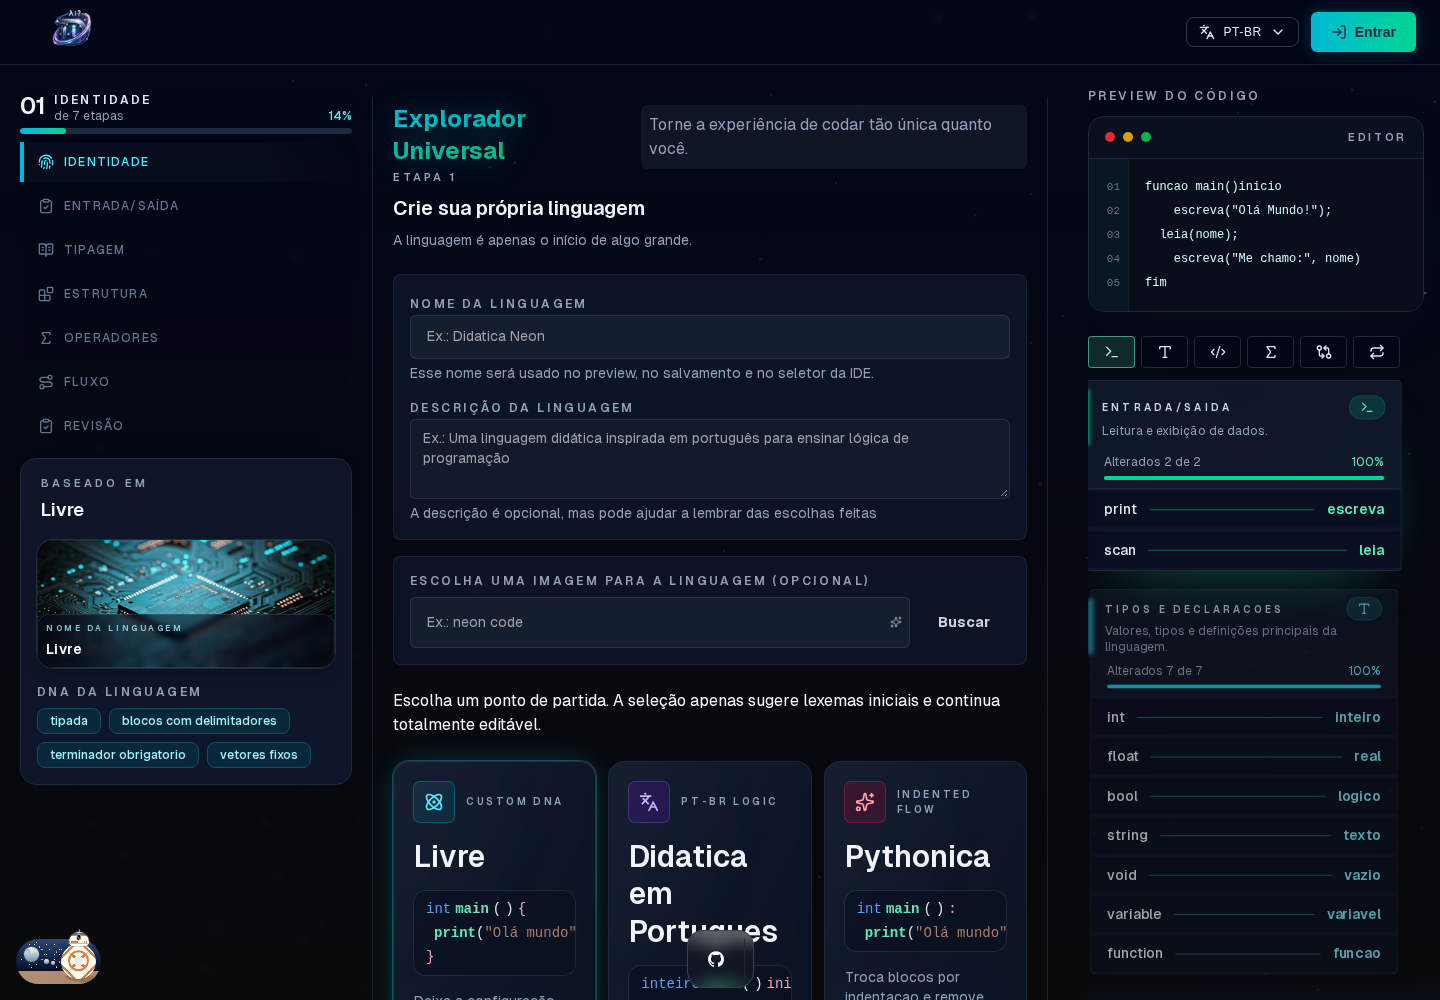
\includegraphics[width=\textwidth,height=0.40\textheight,keepaspectratio]{wizard-desktop-2026-09-16.png}
\caption{Assistente na versão verificada em setembro de 2026, em janela de 1440 por 1000 pixels CSS: etapas na lateral e conteúdo em colunas.}
\label{fig:responsividade-wizard}
\legend{Fonte: captura local da aplicação, sem autenticação.}
\end{figure}

Com a janela de 390 pixels, as etapas passam para uma linha no alto da tela e os cartões ficam empilhados, como mostra a Figura~\ref{fig:responsividade-wizard-celular}.

\begin{figure}[H]
\centering
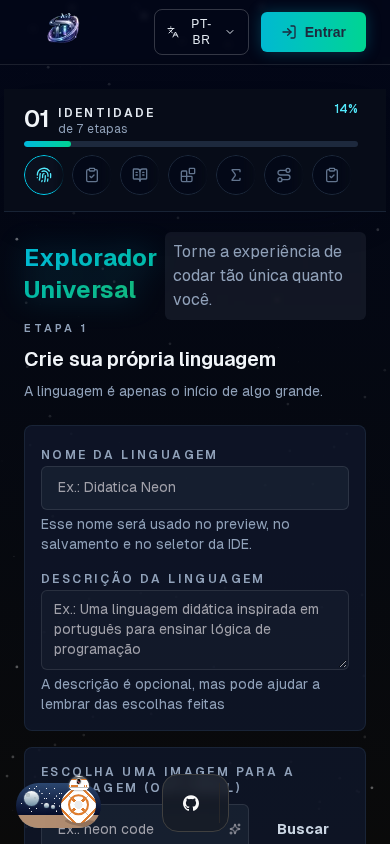
\includegraphics[height=0.32\textheight,keepaspectratio]{wizard-mobile-2026-09-16.png}
\caption{Assistente na versão verificada em setembro de 2026, em janela de 390 por 844 pixels CSS: etapas em linha e cartões empilhados.}
\label{fig:responsividade-wizard-celular}
\legend{Fonte: captura local da aplicação, sem autenticação.}
\end{figure}

A Tabela~\ref{tab:verificacao-axe} resume as ocorrências reportadas pelo axe por regra e cenário. Uma ocorrência corresponde a um elemento identificado pela ferramenta; as contagens de cenários distintos não devem ser somadas como problemas únicos. O relatório também contém itens inconclusivos, sobretudo de contraste, que requerem inspeção manual.

\begin{table}[htbp]
\centering
\caption{Ocorrências reportadas pelo axe no recorte do assistente.}
\label{tab:verificacao-axe}
\footnotesize
\renewcommand{\arraystretch}{1.2}
\begin{tabular}{|p{6.3cm}|c|c|c|c|}
\hline
\textbf{Regra} & \textbf{Claro} & \textbf{Claro} & \textbf{Escuro} & \textbf{Escuro} \\
 & 1440 & 390 & 1440 & 390 \\\hline
Botão sem nome acessível & 1 & 1 & 1 & 1 \\\hline
Contraste insuficiente & 2 & 14 & 5 & 5 \\\hline
Título de documento ausente & 1 & 1 & 1 & 1 \\\hline
Link sem nome acessível & 0 & 0 & 0 & 0 \\\hline
Elementos interativos aninhados & 6 & 6 & 6 & 6 \\\hline
Região rolável sem foco & 3 & 0 & 3 & 0 \\\hline
Alvo de interação pequeno & 1 & 1 & 1 & 1 \\\hline
\end{tabular}
\legend{Fonte: relatório automatizado da verificação de 16 de setembro de 2026.}
\end{table}

Esses achados impedem tratar a acessibilidade como requisito concluído. A aprovação da transição por teclado mostra apenas que os dois passos testados são acionáveis nesse contexto. Permanecem necessárias a correção e a inspeção dos problemas reportados, a verificação do foco visível e dos diálogos, a análise de outras páginas e testes com tecnologias assistivas, conforme a proposta da Seção~\ref{sec:protocolo-avaliacao}. O \textit{script} e o relatório estruturado da verificação estão no repositório do projeto (Apêndice~\ref{ap:repositorio}), nos diretórios \texttt{qualificacao/igor/scripts} e \texttt{qualificacao/igor/verificacao}.

